\documentclass[tikz]{standalone}
\usepackage{pgfplots}
\pgfplotsset{compat=1.15}
\usepackage{mathrsfs}
\usetikzlibrary{arrows,calc}
\usepackage{tkz-euclide}

\usepackage{fp}
\pagestyle{empty}

\definecolor{AngleClr}{rgb}{0,0.39215686274509803,0}
\definecolor{ShapeClr}{rgb}{0.6,0.2,0}
\definecolor{ParacircleClr}{RGB}{217,185,7}

\begin{document}

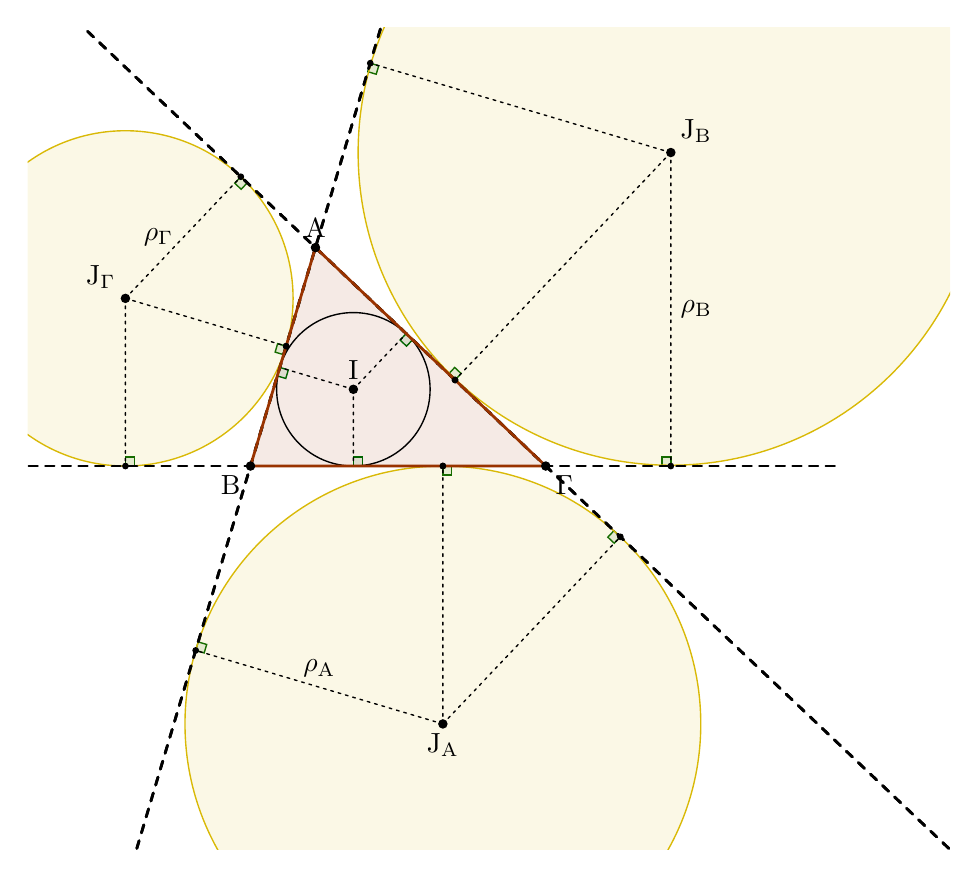
\begin{tikzpicture}[scale=.75]
\tkzSetUpLine[line width=1pt,color=black]
\tkzSetUpPoint[fill=black]

\tkzDefPoints{0/0/B,1.1/3.7/A,5/0/C}

\tkzDefSpcTriangle[ex](A,B,C){Ja,Jb,Jc}
\tkzDefSpcTriangle[extouch](A,B,C){Ta,Tb,Tc}
\tkzDefTriangleCenter[nagel](A,B,C)
\tkzDefCircle[in](A,B,C) \tkzGetPoints{I}{i}

\tkzDefPointBy[projection=onto B--C](I)\tkzGetPoint{IA}
\tkzDefPointBy[projection=onto C--A](I)\tkzGetPoint{IB}
\tkzDefPointBy[projection=onto A--B](I)\tkzGetPoint{IC}

\tkzDefPointBy[projection=onto A--B](Ja)\tkzGetPoint{IA''}
\tkzDefPointBy[projection=onto A--C](Ja)\tkzGetPoint{IA'''}
\tkzDefPointBy[projection=onto B--A](Jb)\tkzGetPoint{IB''}
\tkzDefPointBy[projection=onto B--C](Jb)\tkzGetPoint{IB'''}
\tkzDefPointBy[projection=onto C--A](Jc)\tkzGetPoint{IC''}
\tkzDefPointBy[projection=onto C--B](Jc)\tkzGetPoint{IC'''}

\tkzFillPolygon[fill=ShapeClr,fill opacity=0.1](A,B,C)

\tkzDrawPoints(Ja,Jb,Jc,Ta,Tb,Tc)
\tkzDrawLines[add=1 and 1.75,dashed](A,B)
\tkzDrawLines[add=0.75 and 1,dashed](B,C)
\tkzDrawLines[add=1.75 and 1,dashed](C,A)

\tkzClipBB

\tkzMarkRightAngles[line width=0.5pt, size=.15,color=AngleClr,fill=AngleClr,fill opacity=0.1](Ja,Ta,C Jb,Tb,A Jc,Tc,B Ja,IA''',C Ja,IA'',B Jb,IB'',A Jb,IB''',C Jc,IC'',A Jc,IC''',B I,IA,C I,IB,C I,IC,B)

\tkzDrawCircles[line width=0.5pt,color=black](I,IA)
\tkzDrawCircles[line width=0.5pt,color=ParacircleClr,fill=ParacircleClr,fill opacity=0.1](Ja,Ta Jb,Tb Jc,Tc)

\tkzDrawLines[add=1 and 1.75,dashed](A,B)
\tkzDrawLines[add=0.75 and 1,dashed](B,C)
\tkzDrawLines[add=1.75 and 1,dashed](C,A)
\tkzDrawSegments[line width=0.5pt,color=black,dashed,dash pattern=on 1pt off 1.75pt](Ja,Ta Jb,Tb Jc,Tc Ja,IA'' Jb,IB'' Jc,IC'' Ja,IA''' Jb,IB''' Jc,IC''' I,IA I,IB I,IC)

\tkzDrawPolygon[color=ShapeClr](A,B,C)

\tkzDrawPoints[size=3](Ja,Jb,Jc,I)
\tkzDrawPoints[size=2](Ta,Tb,Tc)
\tkzDrawPoints[size=3](B,C,A)
\tkzDrawPoints[size=2](IA'',IA''',IB'',IB''',IC'',IC''')


\tkzLabelPoint[above](A){$\rm A$}
\tkzLabelPoint[below left](B){$\rm B$}
\tkzLabelPoint[below right](C){$\rm \Gamma$}


\tkzLabelPoint[below](Ja){$\rm J_A$}
\tkzLabelPoint[above right](Jb){$\rm J_B$}
\tkzLabelPoint[above left](Jc){$\rm J_\Gamma$}
\tkzLabelPoint[above](I){$\rm I$}

\tkzLabelSegments[above](Ja,IA''){$\rho_{\rm A}$}
\tkzLabelSegments[right](Jb,IB'''){$\rho_{\rm B}$}
\tkzLabelSegments[left](Jc,IC''){$\rho_{\rm \Gamma}$}

\end{tikzpicture}

\end{document}
